\documentclass[10pt]{article}
\usepackage[utf8]{inputenc}
\usepackage{listings}
\usepackage{xcolor}
\usepackage{subcaption}

\definecolor{codegreen}{rgb}{0,0.6,0}
\definecolor{codegray}{rgb}{0.5,0.5,0.5}
\definecolor{codepurple}{rgb}{0.58,0,0.82}
\definecolor{backcolour}{rgb}{0.95,0.95,0.92}
\usepackage{color}   %May be necessary if you want to color links
\usepackage{hyperref}
\usepackage{graphicx}
\graphicspath{ {./images/} }
\hypersetup{
    colorlinks=true, %set true if you want colored links
    linktoc=all,     %set to all if you want both sections and subsections linked
    linkcolor=black,  %choose some color if you want links to stand out
    urlcolor=blue,
}
\lstdefinestyle{mystyle}{
    backgroundcolor=\color{backcolour},   
    commentstyle=\color{codegreen},
    keywordstyle=\color{magenta},
    numberstyle=\tiny\color{codegray},
    stringstyle=\color{codepurple},
    basicstyle=\ttfamily\footnotesize,
    breakatwhitespace=false,         
    breaklines=true,                 
    captionpos=b,                    
    keepspaces=true,                 
    numbers=left,                    
    numbersep=5pt,                  
    showspaces=false,                
    showstringspaces=false,
    showtabs=false,                  
    tabsize=2
}

\lstset{style=mystyle}


\title{RASD}
\author{Mauro Famà, Giacomo Lombardo}
%\date{October 2021}

\begin{document}
\thispagestyle{empty}
\begin{titlepage}
    \begin{center}
       %\vspace*{2cm}
       {\Huge \textbf{RASD}} %%Replace this with the Title of your research
       \vspace{0.5cm}
       \\
    \begin{LARGE}
        {Requirements Analysis and Specification Document}
        \vspace{1.0cm}
        \\
        
\includegraphics[width=13cm]{polimi.png}
        \vspace{1.5cm}\\
        Mauro Famà (10631287)\\Giacomo Lombardo (10674987)
        \vspace{1.5cm}\\
        {A.Y. 2021/2022}
    \end{LARGE}  
   \end{center}
\end{titlepage}
\newpage
\tableofcontents %this command creates an index
\newpage
\section{Introduction}
As world's population is increasing at steady pace, new challenges arise with its growth.
Accordingly to a recent UN estimate, by 2050 globally there will be almost 10 billion people, 
and food demand is expected to increase between 59\% to 98\%. Furthermore, climate change is causing 
problems to the agriculture that are getting bigger every year: its effect is predicted to result in a 
4\%-26\% loss by the end of the century in the Indian agricuture sector.\\
To tackle the situation, Telangana's state, which is the 11th biggest state in India, has decided to develop a 
platform to implement anticipatory, data-driven models to strengthen the policies in farming, with the ultimate
goal of increasing the output of the agriculture sector.\\
This is the idea behind DREAM (Data-dRiven prEdictive fArMing), a platform where Telangana's
Policy Makers, farmers and agronomists cooperate in order to enhance agriculture performances and facilitate the 
management of help requests, visits to farms and general communications betweens the actors in this scenario.
\subsection{Purpose}
The purpose of this document is to present a detailed description of the DREAM
 (Data-dRiven PrEdictive FArMing) platform. It will explain the purpose and features of 
 the software, the interfaces of the software, what the software will do and the constraints
  under which it must operate. This document is intended for software users and also 
  potential developers. The description will be offered by using models, providing scenarios and 
  their relative use cases, analyzing most important functional and non-functional requirements.
\subsection{Scope} %qui inserirei overview of the function of the system and the reasons for its development, goals and success criteria
The DREAM platform is intended for use by Telengana's policy makers, farmers and agronomists.\\
DREAM allows Telangana's policy makers, through the use of data provided by farmers regarding goods 
production, to extrapolate significative information and obtain a general view of the food production of the entire region. 
In this way, they will be given a platform to model and monitor the region's food system, facilitating the study and the 
realization of an adequate and well-performing long-term production strategy. The platform will provide policy makers the possibility 
to easily monitor farmers' performance and manage agronomists' interventions whenever and wherever needed. 
Furthermore, they will be able to identify those farmers whose production has been particularly good or bad,
in order to reward the best performing farmers with incentives and to provide help to the farmers in need.\\ 
DREAM's goal is also to provide useful resources and tools to local farmers, who will be given a platform to facilitate 
the farmer-to-farmer and farmer-to-policy maker communication. Via DREAM, farmers will be able to participate to forum
discussions, easily create help requests and obtain sensitive information such as accurate weather forecasts and personalized 
suggestions regarding goods and agriculture routines.\\
For what concerns the local agronomists, DREAM facilitates the daily visit controls scheduling and regulates it accordingly
to farmer needs, increasing the visits whether a farmer performance is significantly lower than the average.\\
In this document, the agronomist perspective won't be analyzed in detail, but it will be considered only marginally and in those
cases where there is a significant interaction between agronomists and the other actors.
\subsubsection{Goals}
    \begin{center}
        \vspace{0.5cm}
        \begin{tabular}{|c c|} 
        \hline
        Goal & Description \\ 
        \hline\hline
        G1 & Allow Telangana's Policy Makers to monitor local agriculture\\ 
        \hline
        G2 & Allow farmers to receive assistance or incentives based on their performance\\ 
        \hline
        G4 & Create a farmer's network to promote collaboration and mutual aid \\ 
        \hline
        G5 & Facilitate the management of agronomists's schedules \\ 
        \hline
        \end{tabular}
    \end{center}
\subsubsection{World and Machine Phenomena}
\begin{center}
    \vspace{0.5cm}
    \begin{tabular}{|c c|} 
    \hline
    World Phenomena & Description \\ 
    \hline\hline
    WP1 & Crop damage due to natural causes \\ 
    \hline
    WP2 & Heavy meteorological conditions\\ 
    \hline
    WP3 & Agriculture operations and routines\\ 
    \hline
    WP4 & Agricuture product collection \\ 
    \hline
    WP5 & Control visits to farmers \\ 
    \hline
    \end{tabular}
    \vspace{0.5cm}\\
    \begin{tabular}{|c c c|} 
        \hline
        Shared Phenomena & Description & Controlled By\\ 
        \hline\hline
        SP1 & Insertion of crop collection data & W \\ 
        \hline
        SP2 & Visualization of weather forecasts & M \\ 
        \hline
        SP3 & Visualization of suggestions & M \\ 
        \hline
        SP4 & Sending of notifications by TPMs & W \\ 
        \hline
        SP5 & Receiving of notifications by farmers & M \\ 
        \hline
        SP6 & Sending help requests & W \\ 
        \hline
        SP7 & Contribution to a forum discussion & W \\ 
        \hline
        SP8 & Visualization of crop collection data & M \\ 
        \hline
        SP9 & Interview request & W \\ 
        \hline
        SP10 & Agronomist visit request & W \\ 
        \hline
        SP11 & Login/registration on the platform & W \\ 
        \hline
        \end{tabular}
\end{center}
\subsection{Definitions, Acronyms, Abbreviations}
% PM = Policy Maker
\subsection{Revision history}
\subsection{Reference Documents}
\subsection{Document Structure}
\newpage
\section{Overall Description}
\subsection{Product Perspective}
The system will be implemented from scratch, completely replacing the legacy system.
The system will make use of some already existing functionalities, such as in weather forecasting where there is 
already an existing platform for collecting and visualizing data (https://www.tsdps.telangana.gov.in/aws.jsp).
\subsubsection{Class diagram}
\begin{figure}[ht!]
    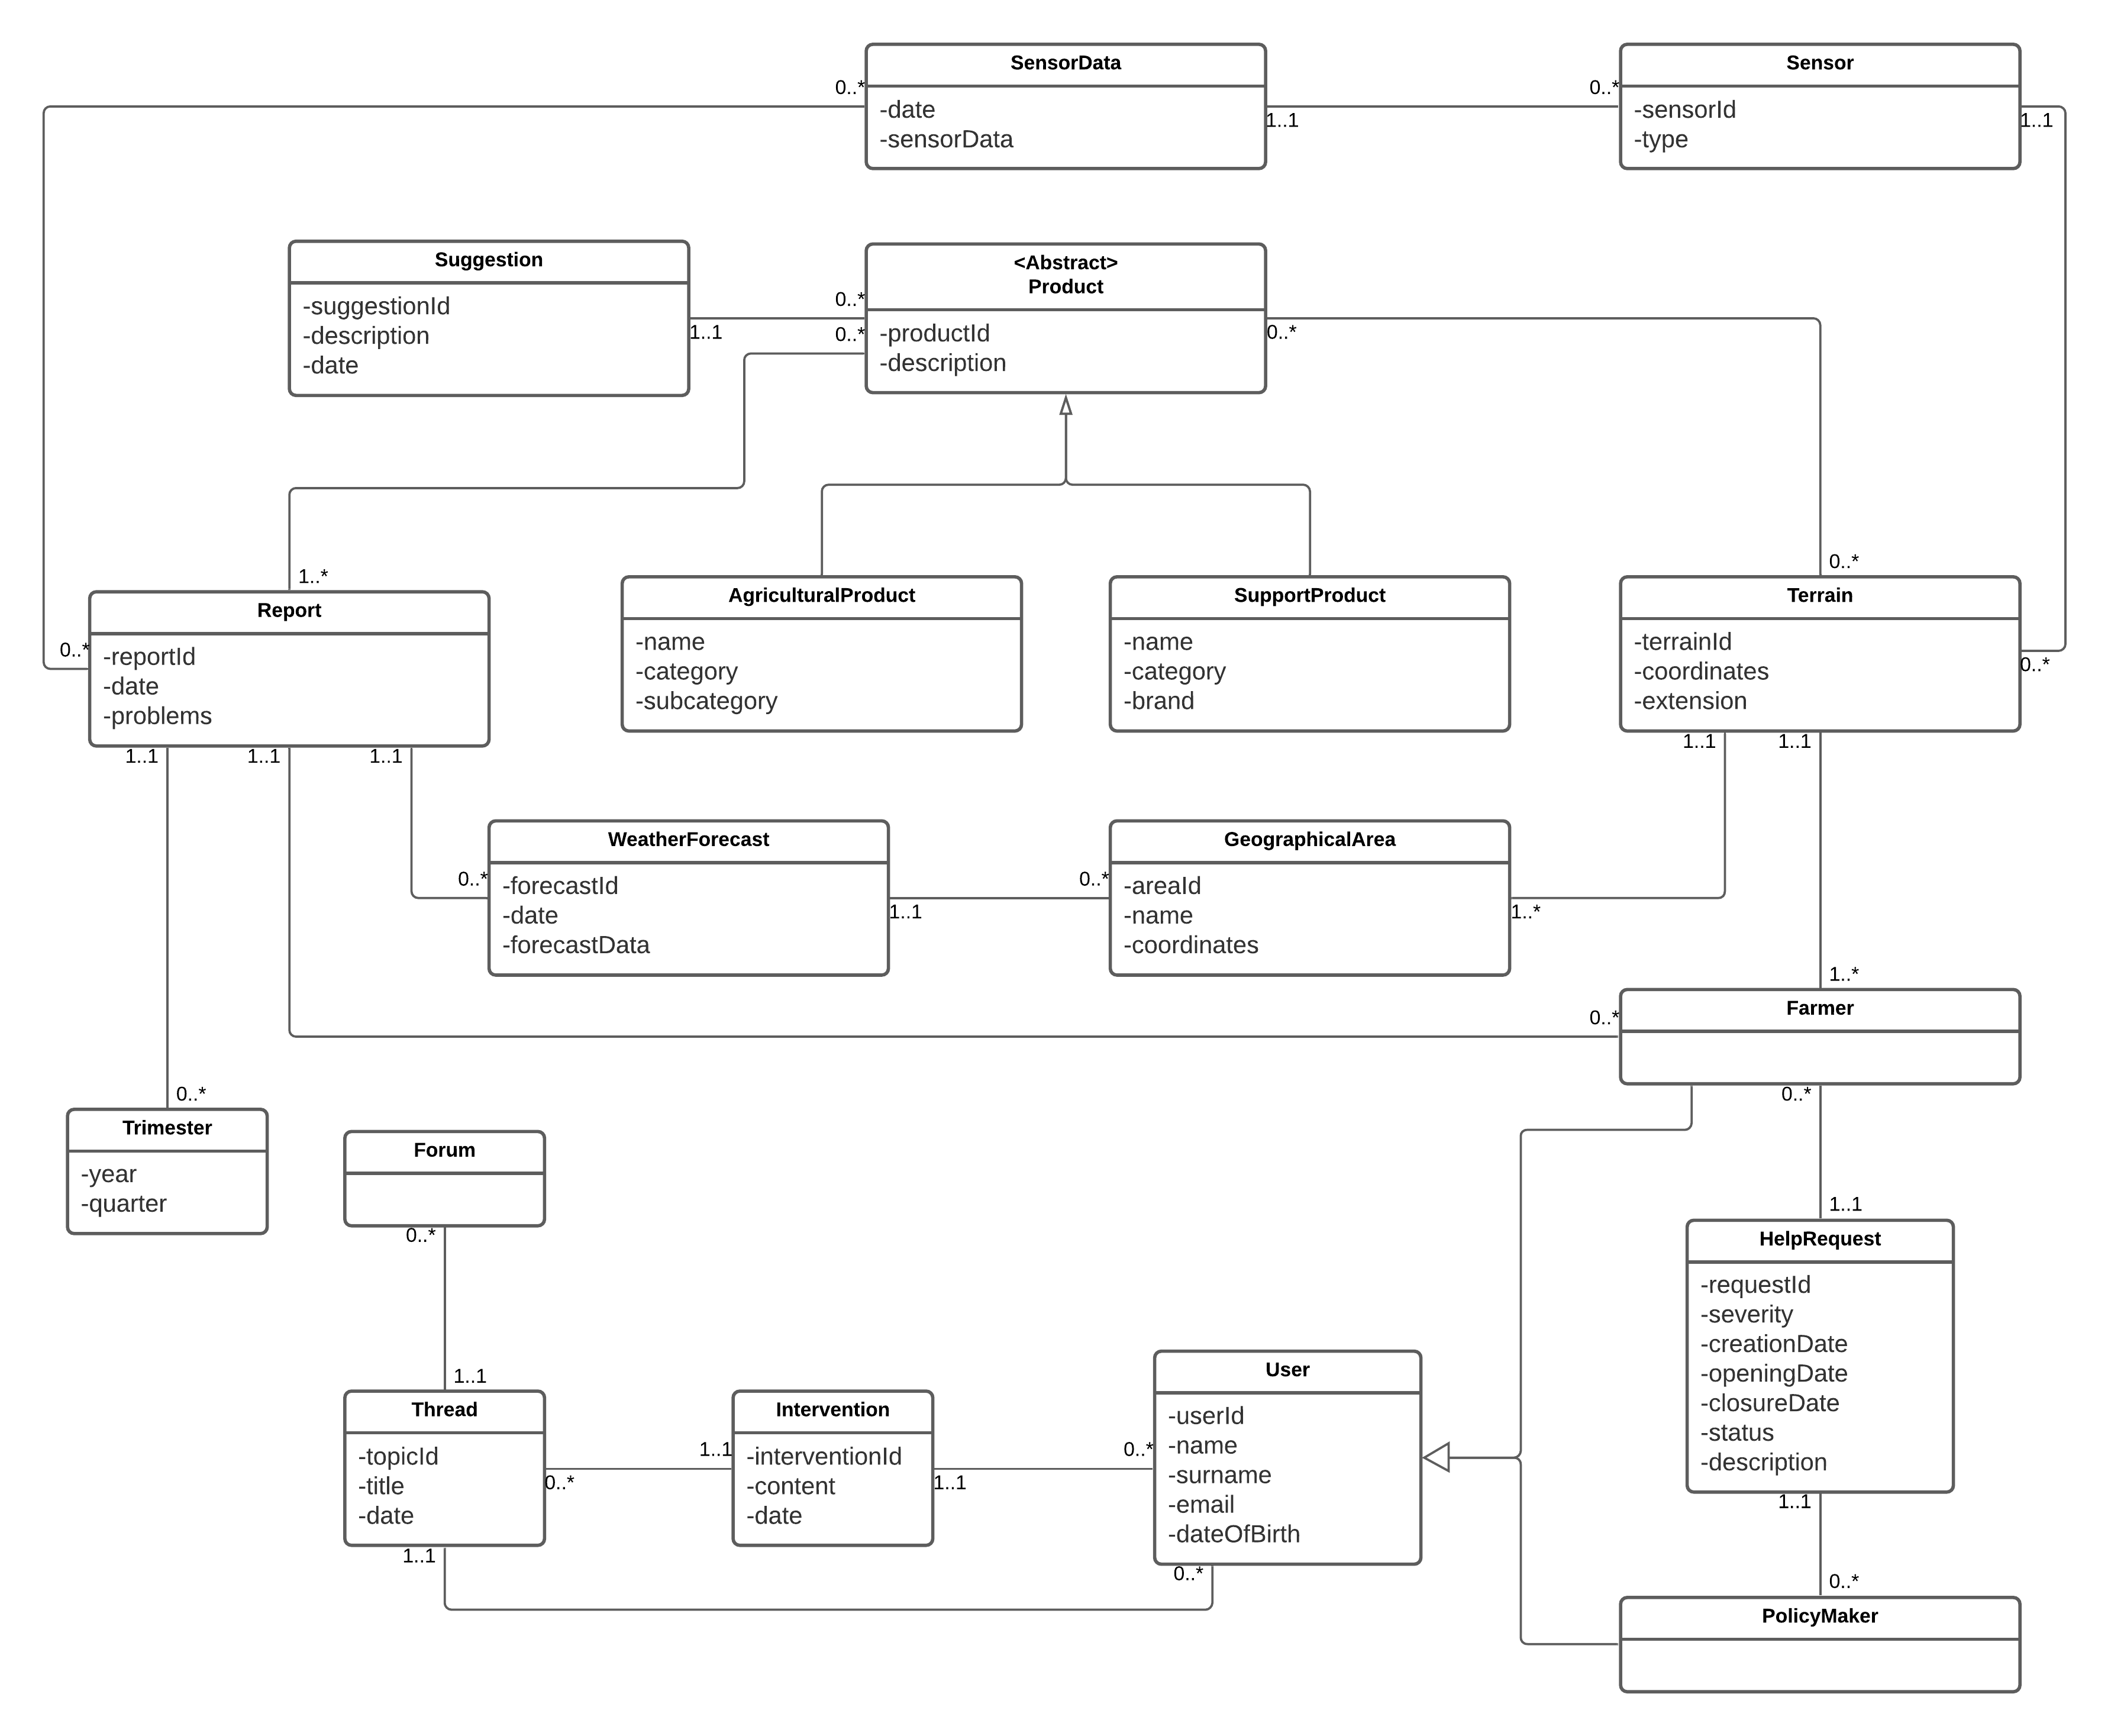
\includegraphics[scale=0.45]{classDiagram.png}
    \caption{Class diagram}
\end{figure}
\newpage
\subsubsection{State diagrams}
\subsection{Product functions}
This section will summarize the main functionalities of the system.
\subsubsection{Farmers registration}
The procedure of registrating farmers into the system will be supervised by policy makers. Local farmers will not be able to register on their own
but, if they intend to participate to the DREAM project, they will request and be provided with the credentials to login into the system. Policy makers will have to 
register the farmer's anagrafical informations and his possessions according to the local registries. Along with the registration in the system, farmers will be provided with
sensors to facilitate the data gathering process: these sensors will be installed by an expert and they will automatically collect additional information about irrigation that 
will be included in periodical reports.
\subsubsection{Agriculture monitoring}
The system will provide Telangana Policy Makers a platform to monitor and manage the local 
agriculture system. Policy makers will be able to visualize relevant data about goods produced by farmers
and will be able to evaluate their performance based on various parameters. The data will be both inserted manually by farmers
(e.g. data regarding the quantity of goods produced) and automatically collected from sensors (e.g. data regarding weather conditions,
soil humidity and irrigation). The system will automatically process the data to provide policy makers a human-friendly
interface where relevant information will be displayed. The UI will display to TPMs both information obtained through data 
aggregation regarding the overall state of local's agriculture and individual information about farmers performance.
In this way, TPMs will be able to identify farmers whose performance has been particularly good or bad and act on them.
\subsubsection{Farmer's assistance}
The system will provide Telangana's local farmers an easy-to-use platform to obtain relevant information and to favor the interaction with TPMs and other farmers.
Farmers will be able to visualize accurate weather forecasts and personalized suggestions regarding the whole goods production process. They will also be able to 
participate in forum discussions with other farmers, favoring collaboration and exchange of knowledge useful to the collectivity.
DREAM will also provide to farmers an easy way to create help requests and send them to TPMs, in order to facilitate and speed-up the support process and favour
interventions where needed. 
Through DREAM, farmers' performance will be monitored by policy makers, and they will be provided assistance if needed. Also, high-performing farmers will be rewarded
with incentives such as prizes, insurances and invitations to excellence programmes.
\subsubsection{Goods production data insertion and analysis}
In order to monitor and visualize information about the local agricuture system, local farmers participating to the DREAM project 
will be requested to provide the system data regarding their production. Goods production data will then be analyzed and will provide TPMs 
useful informations. 
The collected data will regard:
\begin{itemize}
    \item Quantity of goods produced;
    \item Quantity of products used during the process (e.g. fertilizers);
    \item Quantity of water used in irrigation;
    \item Weather conditions;
    \item Soil humidity
\end{itemize}
The system will then process the collected data, calculating parameters used to evaluate farmers' performance. These parameters include:
\begin{itemize}
    \item Amount of water used based on weather conditions;
    \item Resilience to bad weather;
    \item Ambiental impact of used products;
    \item Crop rotation;
    \item and more %e tanti altri ancora! Scoprili tutti!
\end{itemize}
\subsubsection{Scenarios}
\begin{itemize}
    \item \textit{Registration to the DREAM platform}\\ 
    Santosh is a Telangana's local farmer. He receives a letter from the Ministry of Agriculture, Food and Forestry of Telangana containing information
    about the DREAM project. Santosh thinks that he could benefit from the participation to the programme, so he follows the instructions of the letter and
    sends a application to participate to the DREAM project via e-mail to the Ministry. A few days letter his application is accepted and a policy maker sends him
    via e-mail further instructions: he will be provided with credentials to login into the system and an operator will visit his farm to install sensors to monitor
    irrigation. In the meantime the policy maker inserts into the DREAM database the information about Santosh. When Santosh receives the login credentials, he is 
    ready to access to the system and start participating to the project.
    \item \textit{Insertion of crop collection data into the system.}\\ 
    % specificare anche che il farmer inserisce i problemi che ha affrontato
    Rajesh is a Telangana's local farmer. Every morning he wakes up, does a little and poor breakfast and goes to work in the fields.
    Although being a very humble and physically demanding work, agriculture has always been a priority in Rajesh life: nothing gives him
    more satisfaction than seeing the results of his hard work and when he goes to sleep at night, even though he is tired from the long day of work,
    he falls asleep with a smile on his mouth thinking about his crop happily growing in the night. When the crop is ready to be collected, the atmosphere
    is electric in Rajesh's farm: if the crop is good and particularly abundant, all the workers have a big dinner, finely prepared by Rajesh and his wife,
    followed by a long party night where everybody sings and dances. The day after the celebration, Rajesh wakes up with a tremendous hangover, and proceeds
    to login into the DREAM platform. Once he has logged in, he proceeeds to insert into the system the data regarding the collected crop.
    He would have preferred to sleep a few more hours, and only by looking at the computer's screen he gets a big headache, but he carries on, because he
    remembers that tomorrow will be another happy day in the fields of Telangana.
    \item \textit{Awarding of the best performing farmer}\\
    % Assunzioni che ho fatto: ogni policy maker ha un'area di competenza; ogni trimestre sono selezionati
    % 10 agricoltori in base a degli indici definiti dall'alto; a seguito della chiusura del trimestre il sistema
    % memorizza i dati relativi al semestre appena passato e fa partire l'inizializzazione del nuovo trimestre.
    Guepequesh works as PM at the Ministry of Agriculture, Food and Forestry of Telengana. Like every end of the quarter,
     it's time to designate who the top performing farmers of the period were. Guepequesh logs in with his credentials to
      the DREAM portal and goes to his area of expertise, the dashboard shows the ranking of farmers sorted according to 
      the synthetic indices of interest established by the Committee of Policy Makers of Telengana, updated the same day. 
      Guepequesh selects the top 10 farmers shown in the ranking, sends them an email alert stating that they have been 
      selected as the top performing farmers of the quarter, specifying their position in the ranking. The notice contains 
      instructions on how to claim the prizes they have won, and also indicates the dates available for an interview in which 
      the PM will ask the farmer to provide information about the best practices he uses to grow his crops. After notifying 
      all winners, Guepequesh will notify the system to proceed with the closing of the quarter. In the following days, 
      following the interviews, the PM will enter all data related to the best practices followed by the farmer in the system, 
      and they will be forwarded to all farmers in the area who grow the same type of product. 
      \item \textit{Farmers request for help and suggestions by other farmers}\\
      Marrakesh is a young farmer from Telengana. He has recently decided to strike out on his own in the world of agriculture 
      and knows that he will face many challenges. During a normal day's work, Marrakesh notices that even several hours after irrigation, 
      his soil remains very wet and even puddles form. He had never encountered this problem before and decides to rely on the 
      farmers' forum provided by the DREAM platform to which he is subscribed. Marrakesh logs in and goes to the "Problems and Help Requests" 
      section of the forum, creates a new thread and prepares to fill in the required fields for the submission of the request. 
      The young farmer enters a short title, his working area, the type of shoot with which he encountered the problem and an accurate description 
      of the problem he had. All farmers receive a notification on the platform that a new application has been entered, the notification includes 
      the title and type of sprout so that a farmer can immediately determine if he or she considers themselves competent in the field or not. 
      In particular, an experienced farmer named Rastykilo pauses to read the full description of the problem and enters a very accurate 
      response to the problem. All of the farmers who read the response enter positive feedback, and Marrakesh, the next day, feels confident 
      in following Rastykilo's advice, given the many positive feedbacks.
      \item \textit{Identify those farmers who need to be helped as they are performing particularly badly}
      % va inserito? sarebbe molto simile all'awarding ma al posto di premiare li insulta e poi li aiuta
\end{itemize}
\subsection{User Characteristics}
In this section the different types of users of the system will be analyzed. DREAM has three categories of users:
\begin{itemize}
    \item \textbf{Farmers}\\
    Telangana Farmers will mainly use the platform to visualize weather forecasts, insert data about goods production, create help requests and intervene
    in forum discussions. It is safe to assume that most of them will not have much familiarity with this kind of procedures and with
    technological products in general. This requires a UI as simple and intuitive as possible, providing them all the desired functionalities
    without requiring much experience with the system. 
    \item \textbf{Policy Makers}\\
    Telangana Policy Makers will use the platform to monitor and manage the local agriculture. They will perform more complex tasks than farmers, such as 
    visualizing data about performance, interact with farmers and manage help requests and suggestions and agronomists' schedules. We can assume that Policy
    Makers will have at least some experience with the use of management software, and they will be provided more complex functionalities that will require 
    some experience and training with the platform.
    \item \textbf{DREAM system admins}\\
    The DREAM platform will also require administration operations from qualified operators. They will have a robust knowledge of the platform since they will 
    perform system's maintenance and update. They will be designed with this role before the deployment of the system and it won't be possible to register to the 
    platform with this role. 
\end{itemize} 
\subsection{Constraints}
This section contains general observations about boundaries that will limit the system options.
\subsubsection{Regulatory policies}
%da pensarne e aggiungerne, poichè siamo pur sempre in un contesto governativo
\subsubsection{Hardware limitations}
The system will have support a broad list of devices since the end users of the product will be likely
to have basic computers with low performances.
\subsubsection{Interfaces to other applications}
DREAM will implement a pre-existing weather forecasting system, which will be integrated via APIs. Failures in the 
system above will not affect the overall functioning of DREAM but will result in wrong forecasts or in the unavailability of the feature.
\subsection{Domain assumptions}
Domain assumptions define the world in which DREAM works. 
\begin{itemize}
    \item[] \textbf{DA1} Each policy maker has one and one only area to monitor.
    \item[] \textbf{DA2} Terrains cannot be shared: each terrain is associate with one and only farmer. 
    \item[] \textbf{DA3} Farmers have a device able to access the platform. 
    \item[] \textbf{DA4} Farmers always insert correct data in the system.
    \item[] \textbf{DA5} Farmers participating to the programme actively use the platform.
    \item[] \textbf{DA6} Farmers' possessions are already registered at the local Ministry.
    \item[] \textbf{DA7} Policy makers' decisions are solely data-driven and are not affected by personal opinions.
    \item[] \textbf{DA8} Humidity soil sensors are already installed and cover the entire geographical area.
    \item[] \textbf{DA9} Each farmer's terrain humidity data is provided by one and only sensor, associated accordingly to geographical distance from the center of the terrain.
    \item[] \textbf{DA10} Data provided by humidity soil sensors is always correct.
    \item[] \textbf{DA11} Each farmer has an automated irrigation system with a control unit.
    \item[] \textbf{DA12} Each irrigation control unit supports the sensors provided by DREAM.
    \item[] \textbf{DA13} Data provided by the irrigation sensors is always correct.
    \item[] \textbf{DA14} The units of measurement used will always be consistent. 
\end{itemize}
\newpage
\section{Specific Requirements}
\subsection{External Interface Requirements}
\subsubsection{User Interfaces}
\subsubsection{Hardware Interfaces}
% https://iopscience.iop.org/article/10.1088/1742-6596/1339/1/012012/meta se citiamo anche degli articoli accademici è una bella flexata
Different types of hardware interfaces will be required to ensure that the entire infrastructure functions properly.\\
Farmers and PMs will need to have computers connected to the internet and capable of supporting DREAM's dedicated web app.\\
All sensors will have to use IoT technologies, in fact they will necessarily have to be connected to a Wi-Fi module and programmed to create data and send it to the DREAM server. 
\subsubsection{Software Interfaces}
The system will use the external API of the Telengana governmental weather service to collect and transmit data of interest to farmers, depending on their area.\\
The system doesn't provide any API to external application because of the privacy of the farmers.
\subsubsection{Communication Interfaces}
% qui non saprei cosa scrivere
\subsection{Functional Requirements}
\subsubsection{Requirements}
\subsubsection{Goal Mapping on Requirements}
\subsection{Performance Requirements}
Since the system does not need immediate responsiveness, the latency between components can also be in the order of seconds (e.g. 1 to 20 sec).\\
The amount of data produced by IoT sensors is significantly high, the system is expected to be able to process and classify all the data, thus having high storage capacities.\\
\textcolor{red}{To meet these requirements, the system is expected to be distributed in nature and have a Cloud infrastructure to rely on. \%forse non va inserito qua\%}
\subsection{Software System Attributes}
\subsubsection{Availability}
The target is to achieve an improved level of resilience with semi-automated recovery and to be taken offline for maintenance in agreed windows.
System relies on people that use it during the working hours, moreover, it is not needed to provide very high availability because the system is not strictly related with emergency situations.
According to these assumptions, the system should provide an Availability of 99.5\%.
\begin{center}
    \begin{tabular}{|c c c|} 
    \hline
    Availability \% & Downtime per year & Downtime per month\\ 
    \hline
    99.5\%  & 1.83 days & 3.6 hours\\ 
    \hline
    \end{tabular}
\end{center}
\subsubsection{Reliability}
The operations performed must be executed as intended as frequently as possible, in fact the probability that the data displayed is correct must be 
very high, so as not to compromise the evaluations performed by the actors in the system. To meet these requirements, the reliability of the system must 
not be less than 99.97\%.
\begin{center}
    \begin{tabular}{|c c c|} 
    \hline
    Reliability \% & Downtime per year & Downtime per month\\ 
    \hline
    99.97\%  & 2.63 hours & 13.14 minutes\\ 
    \hline
    \end{tabular}
\end{center}
\subsubsection{Security}
The data entered into the platform needs to be protected as it contains confidential information about telengana farmers. A secure communication channel and encryption of messages will be necessary.\\
Operations will always need to be authorized with an authentication mechanism, specifically the PM login mechanism must be 2FA (two-factor authentication).
\subsubsection{Maintainability}
The infrastructure needs thorough documentation of the code base to ensure that the underlying logic can be quickly understood by maintenance personnel.\\
Through the use of design patterns and best practices in the implementation, it will be easier to ensure future additions.
\subsubsection{Portability}
The client application, including the front-end and user interface, must be supported by Windows and Mac operating systems. \\
A mobile version of the client application is not planned.
\end{document}
 